\begin{frame}{Attention we just saw in image captioning}
    \begin{itemize}
        \setlength{\itemsep}{-0.5em}
        \item Previously, we saw how attention helps image captioning models focus on important regions, generating more relevant captions.
        \item However, we noticed limitations—attention sometimes misses subtle details or struggles with complex scenes.
    \end{itemize}
    \begin{figure}
        \centering
        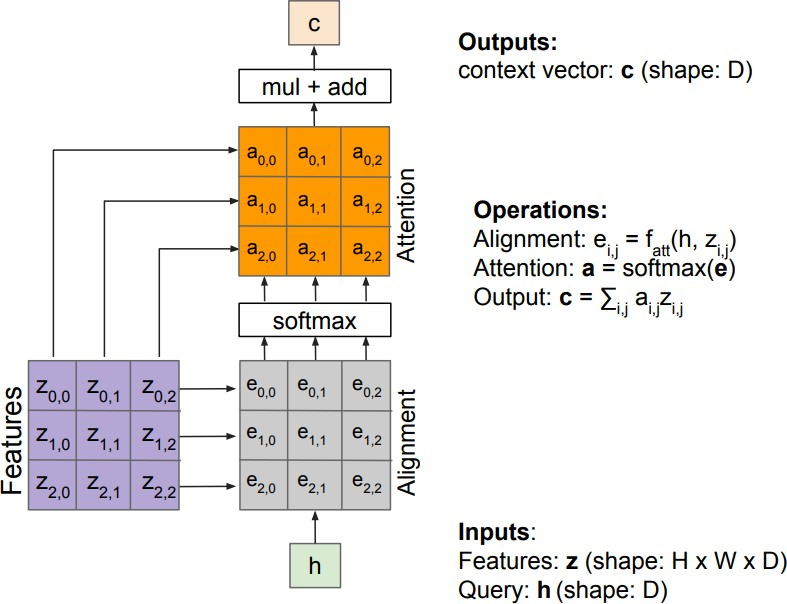
\includegraphics[width=\linewidth,height=0.7\textheight,keepaspectratio]{images/transformers/slide_34_1_img.jpg}
    \end{figure}
\end{frame}


\begin{frame}[allowframebreaks]{General Attention Layer}
    \begin{columns}
    \begin{column}{0.6\textwidth}
        \begin{figure}
            \flushleft
            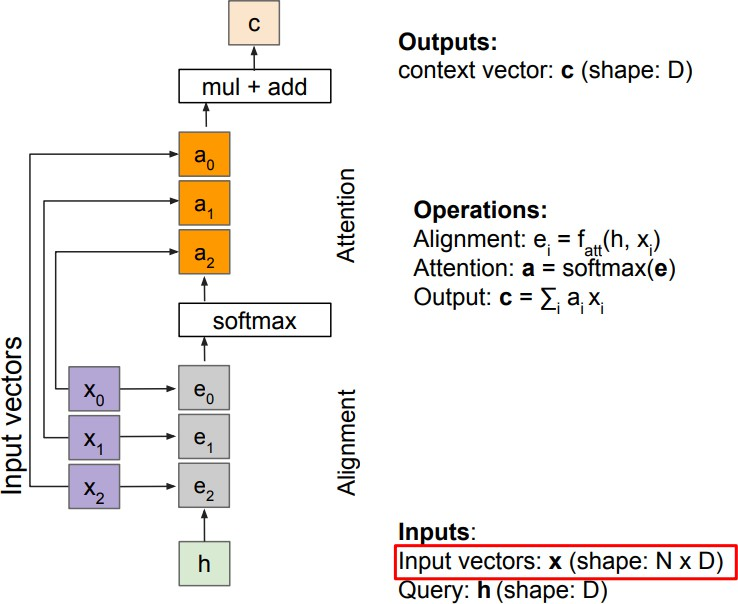
\includegraphics[width=\linewidth,height=\textheight,keepaspectratio]{images/transformers/slide_35_1_img.jpg}
        \end{figure}
    \end{column}
    \begin{column}{0.4\textwidth}
        \begin{itemize}
            \item The \textbf{attention} operation is permutation invariant.
            \item It does not depend on the ordering of features.
            \item Reshape the input of size $H \times W = N$ into $N$ feature vectors.
        \end{itemize}
    \end{column}
    \end{columns}

    \framebreak

    \begin{columns}
    \begin{column}{0.5\textwidth}
        \begin{figure}
            \flushleft
            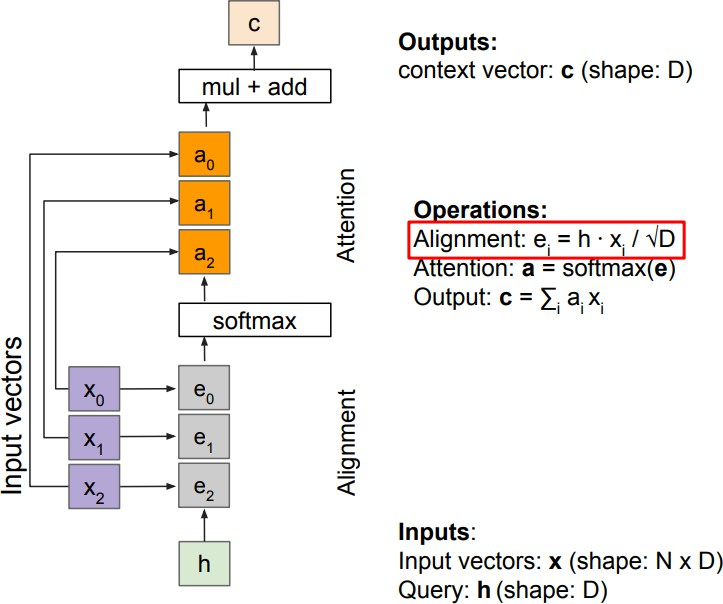
\includegraphics[width=\linewidth,height=\textheight,keepaspectratio]{images/transformers/slide_36_1_img.jpg}
        \end{figure}
    \end{column}
    \begin{column}{0.65\textwidth}
        \begin{itemize}
            \item The original attention mechanism $f_{att}(.)$ uses a simple dot product to compute similarity between queries and keys.
            \item As the feature dimension $D$ increases $\rightarrow$ the dot product sum involves more terms $\rightarrow$ larger variance in the resulting logits.
            \item Larger magnitude vectors produce higher logits $\rightarrow$ causing the softmax output to become more peaked (lower entropy, assuming logits are $IID$).
            \item This means the \textbf{model may focus too narrowly}, assigning very \textbf{high attention to a few positions} and \textbf{almost none to others}.
            \item To counteract this $\rightarrow$ we scale the dot product by dividing by $\sqrt{D}$.
            \item This normalization keeps the variance of the logits more consistent, resulting in a softer, more balanced attention distribution.
        \end{itemize}
    \end{column}
    \end{columns}

    \framebreak

    \begin{columns}
    \begin{column}{0.6\textwidth}
        \begin{figure}
            \flushleft
            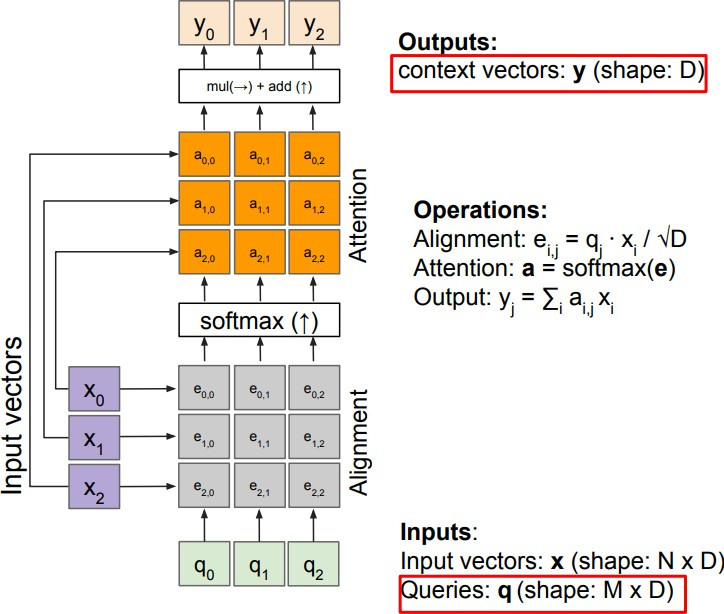
\includegraphics[width=\linewidth,height=\textheight,keepaspectratio]{images/transformers/slide_37_1_img.jpg}
        \end{figure}
    \end{column}
    \begin{column}{0.4\textwidth}
        \begin{itemize}
            \item We can use multiple \textbf{query vectors} in the attention mechanism.
            \item Each query attends to the input independently, producing its own output context vector.
            \item This allows the model to extract different types of information from the same input, enabling richer and more flexible representations.
        \end{itemize}
    \end{column}
    \end{columns}

    \framebreak

    \begin{columns}
    \begin{column}{0.6\textwidth}
        \begin{figure}
            \flushleft
            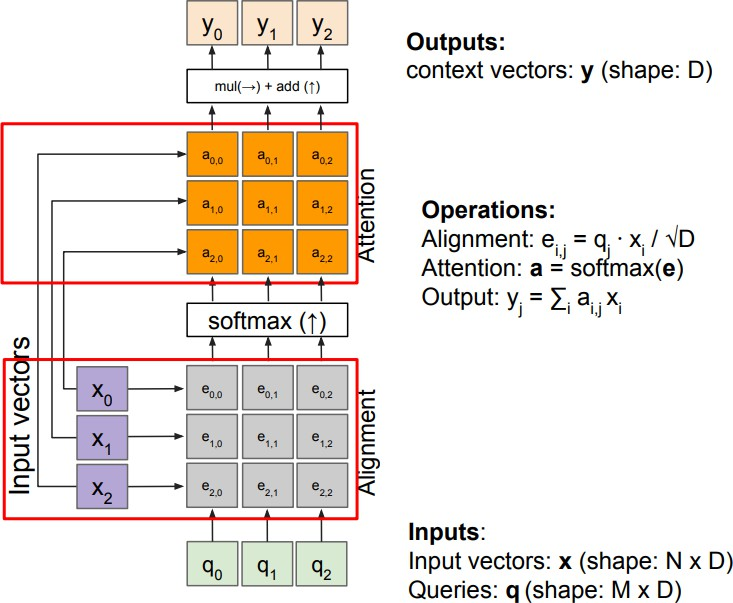
\includegraphics[width=\linewidth,height=\textheight,keepaspectratio]{images/transformers/slide_38_1_img.jpg}
        \end{figure}
    \end{column}
    \begin{column}{0.4\textwidth}
        \begin{itemize}
            \item Observe that the same input vectors are used for both computing the alignment scores (queries and keys) and for generating the attention-weighted output (values).
            \item This dual use lets the model efficiently use the same features for both attending and aggregating information.
        \end{itemize}
    \end{column}
    \end{columns}

    \framebreak

    \begin{columns}
    \begin{column}{0.6\textwidth}
        \begin{figure}
            \flushleft
            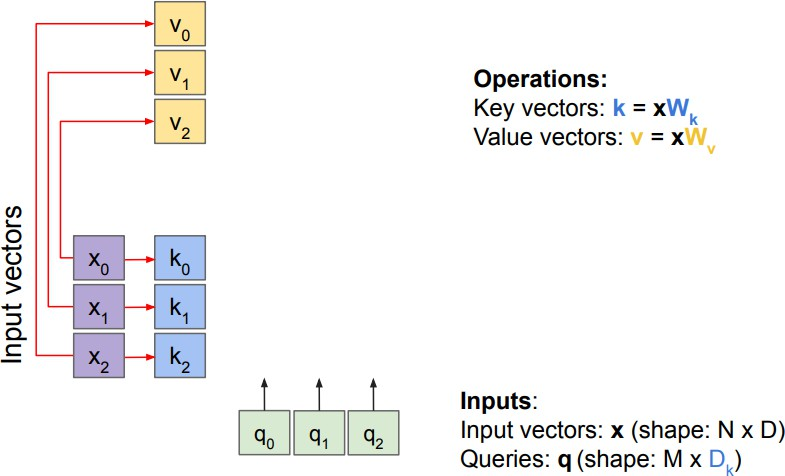
\includegraphics[width=\linewidth,height=\textheight,keepaspectratio]{images/transformers/slide_39_1_img.jpg}
        \end{figure}
    \end{column}
    \begin{column}{0.5\textwidth}
        \begin{itemize}
            \item Notice that the same input vectors are used for both computing alignment scores (as queries and keys) and for generating the attention-weighted output (as values).
            \item To increase the expressiveness of the attention layer, we can introduce separate fully connected (FC) layers before each step $\rightarrow$ one for queries, one for keys, and one for values.
            \item This allows the model to learn different transformations for each role, enabling richer and more flexible representations.
        \end{itemize}
    \end{column}
    \end{columns}

    \framebreak

    \begin{columns}
    \begin{column}{0.6\textwidth}
        \begin{figure}
            \flushleft
            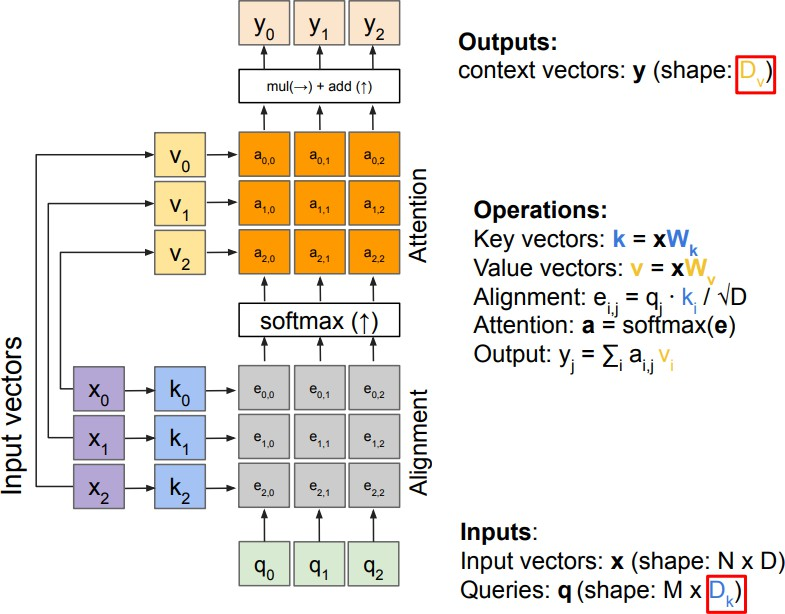
\includegraphics[width=\linewidth,height=\textheight,keepaspectratio]{images/transformers/slide_40_1_img.jpg}
        \end{figure}
    \end{column}
    \begin{column}{0.5\textwidth}
        \begin{justify}
            \begin{itemize}
                \item The input vectors are used for both computing alignment scores (as queries and keys) and for generating the attention-weighted output (as values).
                \item To enhance the expressiveness of the attention layer, we introduce separate fully connected (FC) layers for queries, keys, and values.
                \item Each FC layer can learn a different transformation, allowing the model to capture more complex relationships.
                \item With this setup, the input and output dimensions can differ, depending on the transformations applied by the key and value FC layers.
            \end{itemize}
        \end{justify}
    \end{column}
    \end{columns}
    
\end{frame}